\section{Metodi di tracking basati su modelli} \label{modelTracking}
Il \textit{video tracking} è il processo secondo il quale si localizza un oggetto in movimento all'interno di uno stream video e rappresenta uno dei più interessanti problemi di \textit{computer vision}. Esistono svariati approcci al video tracking, ognuno orientato ad ottimizzare le prestazioni relativamente al campo d'azione. In questo lavoro è stato scelto di effettuare il tracking secondo l'approccio basato su modelli, che viene eseguito secondo due passi fondamentali: la localizzazione dell'oggetto da tracciare ed il tracciamento effettivo.

Il primo passo, computazionalmente non molto oneroso, è stato realizzato tramite il \textit{background subtraction} (descritto nella sezione \ref{sec:bgsub}) e consiste nella rilevazione dell'oggetto all'interno dell'immagine e nell'ottenimento delle informazioni relative.

Il secondo passo, ovvero l'applicazione del tracking al video, rappresenta il punto di maggior interesse del lavoro in quanto consiste nell'elaborazione di una stima della posizione al frame successivo dell'oggetto selezionato; l'esecuzione si basa sull'elaborazione dei dati ottenuti dal processo di localizzazione dell'oggetto.

Gli obiettivi di questo elaborato sono la realizzazione, l'analisi e la comparazione dei due più importanti algoritmi di tracking basato su modelli: il filtro di Kalman, conosciuto in letteratura sin dalla fine degli anni '50 (sarà descritto nella sezione \ref{kalman}) e , ed il Condensation, decisamente più recente rispetto al primo, riconducibile alla fine degli anni '90 (descritto nella sezione \ref{condensation}).

%\textbf{Questa parte va espansa mettendo un po' di discorsi sul tracking generale e poi andando a parare sul tracking model based}

\subsection{Kalman Filter}\label{kalman}
Il Kalman Filter\cite{kalman-intro} è un efficiente filtro ricorsivo che valuta e stima lo stato di un sistema dinamico sulla base di una serie di misure soggette a rumore. Il filtro è molto potente in quanto supporta la stima degli stati passati, presenti e futuri del sistema anche quando la natura del sistema è sconosciuta. \'E usato in molti campi ingegneristici, che vanno dall'applicazione in tecnologie radar all'applicazione in computer vision, come utilizzato in questo stesso ambito.
\subsubsection{Definizione del modello}\label{modelKalman}
Il filtro ha l'obiettivo di stimare lo stato $x \in \Re^n$ di un processo a tempo discreto governato dalla seguente equazione alle differenze
\begin{equation}\label{eq:x}
 x_k=Ax_{k-1}+Bu_{k-1}+w_{k-1}
\end{equation} 
dove 
\begin{description}
 \item [$A$] è la matrice di transizione del modello, ed è applicata allo stato precedente $x_{k-1}$; è quindi una matrice quadrata che mette in relazione due vettori delle stesse dimensioni: lo stato al tempo $k-1$ e lo stato al tempo $k$. Risulta la responsabile dell'aggiornamento dello stato.
\item [$B$] è la matrice di controllo sull'input del sistema. \'E applicata al vettore di controllo $u_{k-1} \in \Re^l$ e mappa questo nella dimensione dello stato $x$; è quindi una matrice rettangolare $nxl$.
\item [$w_k \in \Re^n$] è il rumore che affligge il processo. Si assume che sia descritto da una gaussiana a media $0$ e covarianza descritta dalla matrice $Q_k$. Formalmente $w_k \sim N(0,Q_k)$.
\end{description}

Al tempo $k$ l'osservazione dello stato reale $x_k$ è effettuata tramite il vettore della misura $z \in \Re^m$ che è modellato da
\begin{equation}\label{eq:z}
z_k=Hx_k+v_k
\end{equation}
dove 
\begin{description}
 \item [$H$] è la matrice che mappa lo spazio dello stato reale nello spazio dello stato osservato e risulta per questo rettangolare, di dimensione $mxn$.
\item [$v_k \in \Re^m$] è il rumore dell'osservazione, che come per il rumore $w_k$ è descritto da una gaussiana a media zero e covarianza $R_k$. Formalmente si può esprimere come $v_k \sim N(0,R_k)$.
\end{description}
 Da notare che lo stato iniziale ed i vettori che descrivono la presenza di rumore negli stati successivi sono da considerarsi mutualmente indipendenti.

Come detto in precedenza il filtro di Kalman è un estimatore ricorsivo: questo significa che il filtro applica la sua stima dello stato del processo ed ottiene un feedback nella forma del vettore della misura, dal quale può aggiornare la sua computazione. 

Le equazioni del filtro sono raggruppabili in due macrocategorie: \textit{time-update}, responsabili della proiezione nel tempo dello stato corrente per ottenere la stima a priori dello stato successivo (rappresentata dal vettore $\hat{x}_k^- \in \Re^n$), e \textit{measurement-update}, responsabili dell'incorporazione della misura allo stato corrente nella stima a priori, ottenendo così la stima a posteriori (rappresentata dal vettore $\hat{x}_k \in \Re^n$). 

Solitamente lo stadio relativo al \textit{time-update} viene definito come \textit{predict}, mentre quello relativo al \textit{measurement-update} come \textit{correct}.

\begin{figure}[hb]
\centering
	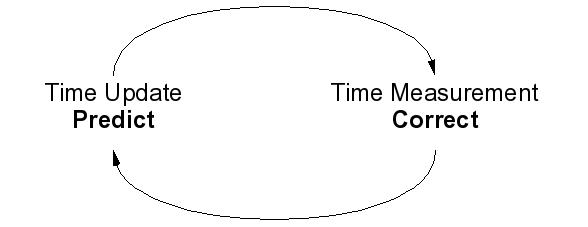
\includegraphics[scale=0.3]{PredCorr.jpg}
\caption{\textit{Il ciclio di calcolo del filtro di Kalman.}\label{fig:predictcorrect}}
\end{figure}
\subsubsection{Predict}
Le equazioni specifiche per il passo di \textit{predict}, che proiettano lo stato e la covarianza dallo stato $k-1$ allo stato $k$ sono 
\begin{equation}\label{eq:prior}
\hat{x}_k^-=A \hat{x}_{k-1}+Bu_{k-1}
\end{equation} 
\begin{equation}
P_k^-=A P_{k-1}A^T+Q
\end{equation} 
dove $A$ e $B$ derivano dalla formula (\ref{eq:x}), considerando sempre la covarianza relativa a $w$ come $Q$, mentre $P_k^-$ è una matrice che rappresenta la covarianza sull'errore nella stima a priori e $P_k$ è una matrice che rappresenta la covarianza sull'errore nella stima a posteriori.
\subsubsection{Correct}

Le equazioni che invece formalizzano il passo di \textit{correct} effettuano una stima sul guadagno del filtro tra l'osservazione attuale e quella predetta (\ref{eq:K}), ottengono la stima a posteriori  (equazione (\ref{eq:post})) data la stima a priori effettuata nel passo di update (\ref{eq:prior}) e dall'osservazione dello stato reale, definita in \ref{eq:z}; viene calcolata anche la covarianza sull'errore nella stima a posteriori (\ref{eq:P}):
\begin{equation}\label{eq:K}
K_k = P_k^- K_T(HP_k^-H^T+R)^{-1}
\end{equation} 

\begin{equation}\label{eq:post}
\hat{x}_k=\hat{x}_k^-+K_k(z_k-H\hat{x}_k^-)
\end{equation} 

\begin{equation}\label{eq:P}
P_k=(1-K_kH)P_k^-
\end{equation} 

\subsubsection{Parametri e configurazione del filtro}\label{tuning}
L'esecuzione dell'algoritmo è direttamente dipendente dalla scelta che viene effettuata riguardo ai parametri di configurazione, in particolare dai valori dei componenti delle matrici $Q$ ed $R$.

La matrice che tiene conto della covarianza dell'errore sulla misura, $R$, è generalmente misurata prima dell'applicazione del filtro. Misurare questa grandezza è possibile perchè si suppone di poter misurare il processo in ogni momento, cosicchè possiamo avere anche delle misure ``offline'' con le quali possiamo affinare il calcolo.

La determinazione dei valori della matrice $Q$ invece, è solitamente molto più complicata da ottenere, perchè non c'è la possibilità di osservare direttamente il processo che il filtro sta stimando. 

In entrambi i casi la tecnica solitamente utilizzata per effettuare la stima tramite il filtro di Kalman è di renderlo più performante ``sintonizzando'' i valori di Q ed R e riapplicando il filtro, in modo da determinare empiricamente la miglior configurazione. 

Possiamo notare inoltre che quando nell'esecuzione le matrici $P$ e $Q$ sono costanti, anche la covarianza sull'errore della stima $P_k$ ed il guadagno di Kalman $K_k$ si stabilizzano velocemente fino a rimanere costanti.
\begin{figure}[hb]
\centering
	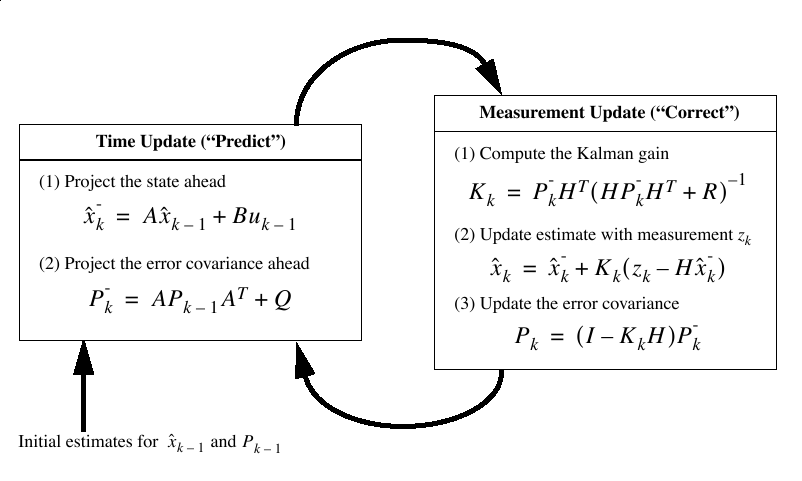
\includegraphics[scale=0.4]{cicloKalman.png}
\caption{\textit{Ciclo di Kalman completo, con parametri ed equazioni}\label{fig:completeKalman}}
\end{figure}

\newpage

\subsection{ConDensation}\label{condensation}
Il ConDensation (\textbf{Con}ditional \textbf{Dens}ity Propag\textbf{ation}) \cite{condensation} è un algoritmo probabilistico molto noto in \textit{computer-vision}, conosciuto anche come Particle Filtering. 

Peculiarità di questo algoritmo è quella di riuscire a stimare e tracciare con precisione i contorni di un oggetto in movimento all'interno di un video, come si può vedere dalla figura \ref{fig:hand}. L'algoritmo risulta ottimo nel tracking di traiettorie non lineari o afflitte da rumore non gaussiano.

\begin{figure}[hb]
\centering
	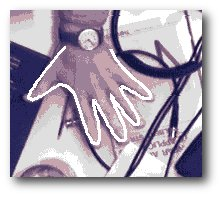
\includegraphics[scale=0.6]{hand.jpg}
\caption{\textit{Esempio di applicazione del ConDensation per la rilevazione del contorno di una mano}\label{fig:hand}}
\end{figure}

Per quanto rigurda il nostro lavoro il Condensation ci interessa perchè risulta robusto rispetto a dati molto rumorosi ed a cambiamenti di stato non lineari. La semplicità di questo permette di utilizzare per la descrizione approssimata del moto dell'oggetto anche modelli dinamici non lineari. In modo particolare è quest'ultima caratteristica che lo contraddistingue in modo netto con il filtro di Kalman, che viceversa raggiunge il massimo della sua efficienza in ambiti lineari. 

L'algoritmo utilizza un campionamento casuale e ordinato per modellare funzioni di densità di probabilità arbitrariamente complesse. Utilizza N campioni pesati per approssimare la curva che descrive la distribuzione dei dati.

Ciascun campione - sample - consiste dunque di uno stato e di un peso. Il peso è proporzionale alla probabilità che lo stato del sample sia lo stato predetto dall'algoritmo.

Chiamiamo con $H_{t}$ il vettore dei samples \{$\overrightarrow{s_1}(t),\overrightarrow{s_1}(t),...,\overrightarrow{s_N}(t)$\} all'istante $t$. (ipotesi)
\begin{equation}
	\overrightarrow{s_i}(t)= \{\overrightarrow{x_i}(t),p(x_i(t))\}
\end{equation}

$\overrightarrow{x_i}(t)$ è la posizione stimata per il sample $i$ all'istante $t$.\\
$p(\overrightarrow{x_i}(t))$ è la probabilità associata alla posizione $\overrightarrow{x_i}(t)$ che caratterizza il sample $i$\\

\textbf{Inizializzazione - passo 0}\\
Al primo passo dell'algoritmo si inizializza tutti i samples:
\begin{itemize}
\item Ciascuna posizione può essere scelta in modo casuale secondo una distibuzione uniforme.
\item La probabilità associata a ciascun sample al primo passo è invece distribuita secondo una gaussiana standard centrata nel valore medio tra il valore massimo e il valore minimo assumibile per la posizione dell'oggetto e la relativa varianza.

\end{itemize}


\textbf{Esecuzione - passo t}\\
Il sample $\overrightarrow{s_i}(t)$ con probabilità maggiore è la predizione per il Condensation.\\

Per passare dal vettore di stato $H_{t}$ al successivo $H_{t+1}$ si eseguono i seguenti passi:
\begin{enumerate}
\item Si campiona la posizione reale dell'oggetto al passo t. [$\overrightarrow{z}(t)$]
\item Si calcola la posizione per ciascun sample secondo lo spostamento dato dal modello dinamico che in qualche modo descrive il moto dell'oggetto: 
\begin{equation}
	$\overrightarrow{x_i}(t+1)$= f($\overrightarrow{x_i}(t)$)
\end{equation}
\item Si stima la probabilità $p(\overrightarrow{z}(t))$ secondo la densità di probabilità che caratterizza i campioni all'istante t.
\item Per ogni sample è ricalcolata la probabilità condizionata applicando il teorema di Bayes:
\begin{equation}
	p_i(\overrightarrow{x_i}(t+1))= p($\overrightarrow{x_i}(t)$\|$\overrightarrow{z}(t)$)
\end{equation}
\end{enumerate}

Il risultato otteenuto è un nuovo set di $N$ \textit{samples} per il tempo $t$.

\begin{figure}[hb]
\centering
	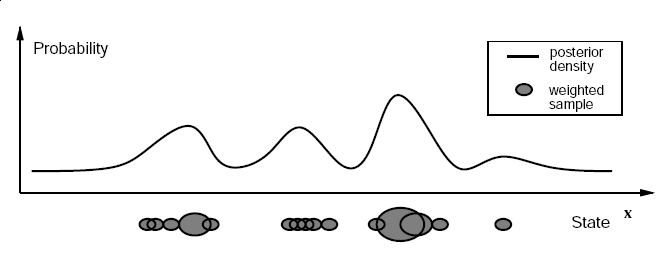
\includegraphics[scale=0.6]{samplesProb.png}
\caption{\textit{Samples e relative probabilità}\label{fig:samplesProb}}
\end{figure}

%%%%%%%%%%%%%%%%%%%
%Meo io mi concentrerie di più su quest ultima parte che viene dove descrivi i modelli piuttosto che sulla teoria del %condensation. quella secondo me può essere fatto più all' acqua di rose.
%%%%%%%%%%%%%%%%%%%
\subsection{Descrizione dell' implementazione dei modelli} \label{sec:modelli}
Solitamente in letteratura si considera come \textit{Modello} la rappresentazione di un oggetto che corrisponda al fenomeno modellato per il fatto  di riprodurne le caratteristiche ed i comportamenti fondamentali. 

Risulta quindi fondamentale riuscire a definire un modello formale il più precisamente possibile, in modo da garantire che l'astrazione matematica dell'evento che vogliamo poi utilizzare per l'esecuzione degli esperimenti sia il più coerente possibile all'entità reale. 

L'obiettivo è stato quello di modellare il moto generico di un oggetto nel piano, per poi riuscire tramite model based tracking a predirne il moto. Inizialmente la modellazione si è basata sull'osservazione del fenomeno fisico della caduta di un grave (\textit{Bouncing Ball}) e sulla successiva scrittura dell sistema dinamico che lo rappresenti a livello teorico. L'attenzione si è poi volta all'estensione del modello costruito per un moto che non fosse solo di caduta verticale, ma che potesse spaziare anche su di un piano con una certa velocità verticale e orizzontale. 

Il modello quindi risulta la rappresentazione formale della posizione del punto di interesse sul piano, della velocità del punto sul piano stesso e quindi dell'aggiornamento della posizione; rispetto al modello iniziale, il modello sul quale sono stati effettuati gli esperimenti è quindi dotato di una strutturazione a due componenti, $x$ ed $y$, piuttosto che una semplice componente verticale.% e di una variabile $g$ che consente di regolare la misura della accellerazione gravitazionale espressa in pixel/s
%\footnote{questa unità di misura deriva dalla unità di misura del video (pixel) riportat al tempo. Quindi per ogni moto andrà fatta la conversione da$ m/s^2$ alla nostra unità $pixel/s^2$}.

Come descritto nella sezione \ref{modelKalman}, il modello si struttura sulla definizione delle matrici e dei vettori alla base delle equazioni \ref{eq:x} e \ref{eq:z}.

L'equazione \ref{eq:x} descrive l'aggiornamento dello stato del modello, rappresentato appunto dal vettore $\overrightarrow{x_k}$ al tempo precedente $\overrightarrow{x_{k-1}}$, del vettore di controllo $\overrightarrow{u_{k-1}}$ e del rumore sul processo $w_{k-1}$. 

Il vettore $x$ risulta essere di dimensione $4 x 1$, della forma 
\begin{equation}\label{eq:vettoreX}
 \overrightarrow{x}=\begin{bmatrix} x \\ y \\ v_x \\ v_y \end{bmatrix}
\end{equation} 

dove ogni componente risulta:
\begin{itemize}
\item $x$ l'ascissa della posizione sul piano cartesiano come rappresentato dalla figura \ref{fig:pianoStato}.
\item $y$ l'ordinata della posizione sul piano cartesiano come rappresentato dalla figura \ref{fig:pianoStato}.
\item $v_x$ la velocità della componente orizzontale.
\item $v_y$ a velocità della componente verticale.
\end{itemize}

Responsabile della mappatura del suddetto stato al tempo $k-1$ verso lo stato al tempo $k$ è la matrice $A$, matrice di transizione del modello, che risulta essere quadrata ($4 x 4$) in quanto mantiene la relazione tra due vettori delle stesse dimensioni.
\begin{equation}\label{eq:matriceA}
 A = 
\begin{bmatrix}
 1 & 0 & \Delta t & 0 \\
 0 & 1 & 0 & \Delta t \\
 0 & 0 & 1 & 0 \\
 0 & 0 & 0 & 1
\end{bmatrix}
\end{equation} 

dove i parametri al suo interno mappano la transizione di ogni componente: rispettivamente le posizioni passate vengono sovrascritte da quelle nuove e lo stato aggiornato dall'equazione $x + \Delta t \cdot v_x$,per ogni riga della matrice.

Il vettore $B$, moltiplicato per il vettore dei controlli esterni $u$, comporta una modifica al sistema solo sull'ultima componente (velocità verticale).\\%, infatti come detto precedentemente, si da la possibilità di poter controllare un' eventuale accelerazione gravitazionale.
Nella realizzazione si è impostato il parametro $g$  e $ \Delta t$ pari ad 1, per tracciare il moto su un piano, in quanto non si avevano forze esterne, che potessero condizionano il sistema. 

\begin{equation}
 B =\begin{bmatrix} 0 \\ 0 \\ 0 \\ g \Delta t \end{bmatrix}\end{equation} 

L'ultima componente della relazione \ref{eq:x} è la modellazione vettoriale del rumore, rappresentata come visto tramite il vettore $w$; assumendo il rumore come gaussiano risulta di interesse la descrizione della matrice che modella la covarianza di questo, rappresentata da $Q$, già descritta nella sezione \ref{tuning} riguardo all'importanza che riveste nella sintonizzazione del filtro di Kalman, come si è ampiamente spiegato nella sezione \ref{sec:esperimenti}~~Esperimenti .

 
\begin{equation}
Q = \begin{bmatrix} 
0.01 & 0 & 0 & 0\\
0 & 0.01 & 0 & 0\\
0 & 0 & 0.01 & 0\\
0 & 0 & 0 & 0.01
\end{bmatrix}\end{equation} 


%Cosa si prende per varianza di uno dell'altro, come è fatto lo stato (vettore di 4 dimensioni di cui 2 posizione xy etc..)


Le ultime due matrici che compaiono nelle equazioni del modello riguardano la misura, cioè i valore ottenuti dal background subtraction. 

La prima ( \ref{eq:matriceH} ) pesa il valore dell'osservazione, effettuata dal background subtraction, per correggere la predizione del filtro di kalman.

\begin{equation} \label{eq:matriceH}
 H = \begin{bmatrix} 
1 & 0 & 0 & 0\\
0 & 1 & 0 & 0
\end{bmatrix}
\end{equation}


La seconda ( \ref{eq:matriceR} ) rappresenta la covarianza associata al rumore nella misura, che nel nostro caso assume i valori sottostanti,molto vicini a zero,data la quasi assenza di rumore nel calcolo della misura.


\begin{equation}\label{eq:matriceR}
 R = \begin{bmatrix} 
0.285 & 0.005\\
0.005 & 0.046
\end{bmatrix} 
\end{equation}

~\\
Il nostro modello viene inserito nell'applicazione combinando l'uso del calcolo matriciale fornito dalle OpenCv con il parsing di un file testuale \texttt{data.txt}, che risulta essere l'input dei dati dell' applicazione.\\

\'E bene sottolineare che questo modello è usato ovviamente il kalman, ma soprattutto la matrice A di transizione dello stato è riutilizzata anche nell'algoritmo ConDensation per ricalcolare i valori dei samples.


Per maggior approfondimento sullo sviluppo, costruzione e progettazione del software si rimanda alla sezione \ref{sec:software}.
